\documentclass[12pt,a4paper,english,twoside]{book}
\usepackage[german,english]{babel}
\usepackage[T1]{fontenc} 
\usepackage[latin1]{inputenc}
\usepackage{amsfonts}
\usepackage{amsmath}
\usepackage{latexsym}
\usepackage{amssymb}
\usepackage{epsfig}
\usepackage{moreverb}
\usepackage{rotating}
\usepackage{enumerate}
\usepackage{graphics, graphicx,wrapfig}
\usepackage{fancybox}
\usepackage{picinpar,varioref,floatflt}
\usepackage{ae}
\usepackage{longtable}
\usepackage{textcomp}
\usepackage{float}
\usepackage{url}
\usepackage{tabularx}
\usepackage{unizhdt-MA}
\usepackage{listings}
\usepackage{caption}
\usepackage{tikz}
\usepackage[thinlines]{easytable}

\colorlet{punct}{red!60!black}
\definecolor{background}{HTML}{EEEEEE}
\definecolor{delim}{RGB}{20,105,176}
\colorlet{numb}{magenta!60!black}


\lstdefinelanguage{json}{
    basicstyle=\fontsize{8}{8}\selectfont\ttfamily,
    numbers=left,
    numberstyle=\scriptsize,
    stepnumber=1,
    numbersep=8pt,
    showstringspaces=false,
    breaklines=true,
    frame=lines,
    %backgroundcolor=white,
    literate=
     *{0}{{{\color{numb}0}}}{1}
      {1}{{{\color{numb}1}}}{1}
      {2}{{{\color{numb}2}}}{1}
      {3}{{{\color{numb}3}}}{1}
      {4}{{{\color{numb}4}}}{1}
      {5}{{{\color{numb}5}}}{1}
      {6}{{{\color{numb}6}}}{1}
      {7}{{{\color{numb}7}}}{1}
      {8}{{{\color{numb}8}}}{1}
      {9}{{{\color{numb}9}}}{1}
      {:}{{{\color{punct}{:}}}}{1}
      {,}{{{\color{punct}{,}}}}{1}
      {\{}{{{\color{delim}{\{}}}}{1}
      {\}}{{{\color{delim}{\}}}}}{1}
      {[}{{{\color{delim}{[}}}}{1}
      {]}{{{\color{delim}{]}}}}{1},
}


%%%%%%%%%%%%%%%%%%%%%%%%%%%%%%%%%%%%%%%%%%%%%%%%%%

% Define the language of the diploma thesis
\selectlanguage{english}
%\selectlanguage{german}

\pagestyle{headings}

\begin{document}

%%%%%%%%%%%%%%%%%%%%%%%%%%%%%%%%%%%%%%%%%%%%%%%%%%

% Define the author printed on the cover page
\author{Sebastian Sanchez}
% Define the city and country of the author
\authorcity{Z\"urich, Switzerland}
% Define the student ID (Matrikelnummer)
\studentid{17-732-710}
% Define the title with optional subtitle
%\title{DialogFlow Chatbot for Intent Aware in Security}
\title{An Intent-Aware Chatbot for Cybersecurity Recommendation} % Suggestion - Also, you can define a name for the Chatbot
% Define the supervisors
\supervisors{Muriel Franco, Eder Scheid}
% Define the submission date
\submissiondate{February 30, 2019}

%%%%%%%%%%%%%%%%%%%%%%%%%%%%%%%%%%%%%%%%%%%%%%%%%%

% Make the title page
\maketitle

% Make the imprint on the back of the cover page
\makeimprint

\pagenumbering{roman}

% Include the files of the diploma thesis
%\cleardoublepage
\chapter*{Abstract}
\addcontentsline{toc}{chapter}{Abstract}
\selectlanguage{english}
Nowadays the cloud architecture is a growing trend that allow us to scale systems without having a physical architecture. This seems to be the future but it also presents several challenges for the current IT System Administrators since cyber attacks are on the growth and the need for performance and availability is also on the growth. In order to mitigate this problem we created a ChatBot using DialogFlow that gathers information from the System Administrator and maps the requirements using pretrained Machine Learning models that use Natural Language Processing to identify and match possible requirements in a few layers of questions using the available System Administrator Tooling such as IPTables, Firewalls, DDoS Managers and so on. The tool will also feature a client that will retrieve the data and further process it using the described architecture to generate a data structure that other tools could use to execute the recommended solutions or to expand into them.
%\cleardoublepage
\chapter*{Acknowledgments}
\addcontentsline{toc}{chapter}{Acknowledgments}

To Muriel Franco my thesis supervisor who guided me throughout the process and provided guidelines and support to overcome issues. Also, I would like to thank the Communications System Group to allow take place in the research with the group and the support throughout the process and presentations.

Finally, Would like to thank {reviewers, family, friends expand here}

\tableofcontents

\cleardoublepage
\pagenumbering{arabic}
\chapter{Introduction}
Cybersecurity has proven to be a key player in the digital era and, thus, an important matter to any company or government that needs to use or provide online services. The investments in cybersecurity have been arising along the years to which is expected to exceed \$124 billion USD in 2019 in order to contract cloud-based security services \cite{GrowthForecast}. However, there is no generic answer to the best way to defend against cyberattacks, since the protections offered can differ from several aspects (e.g., price, technology, performance, and supported cyberattacks). Thus, the process of decide for one cybersecurity solution or configurations is a hard task, mainly when there are no cybersecurity experts in a company.

Based on that, recommender systems with simplified interfaces can help end-users to understand the most suitable cybersecurity solution based on his real demands. However, there is a lack of this kind of system that might not be able only to identify the best solution for a network attack but also guide the end-user for possible configurations and tasks to be done in order to prevent and mitigate a cyberattack.

In order to take advantage of this system, a broad scope of possible solutions can be provided based on the existing state-of-the-art technologies such as Software-defined Networking (SDN), Network Functions Virtualization (NFV), and machine learning. Such technologies can be, for example, a base for tools that could be an issue to protect against different cyberattacks. Therefore, information from the underlying infrastructure, cyberattacks characteristics, and end-users profiles can be used as input to help in a way that eases the task of planning and protection of its business. For that, different mechanisms can be explored to create a human-computer interface where information can be obtained directly from the end-user.

In such a direction, several studies have found ways to interact in a more natural way using chatbots \cite{networkIntents} to map text to intents that might suggest the solution for a common or already experienced network problem. This is a guideline proposed as an accepted enhancer of the interaction between end-users and recommender systems to benefit different cybersecurity aspects. DialogFlow Chatbot, for example, can be used to map the needs of end-users using Natural Language Processing (NLP) to generate a structure that is capable of providing enough abstraction to be used by cybersecurity recommender systems like that introduced in \cite{MENTOR}.

\section{Motivation}
At the current state-of-the-art, there is a tendency to grow in the cloud-based services. As discussed in \cite{growth2}, the expected annual growth of the cloud computing services is about 27\% annually starting from 2018. Thus the amount of the network operators needed would be defied from the market study tendency, which shows a growth of only 24\% in computer science careers across the US \cite{computerScienceStudents}. This will undoubtedly culminate in an increasing tendency for network operators and sysadmins, which are educated to handle security issues such as cyberattacks, performance issues, or business availability. At the same time, there is a growing tendency of cyberattacks as described by [REF], thus meaning that measures to guarantee security aspects must be maintained while taking into account the limited amount of people capable of maintaining the security of a system. Thus, there are opportunities to design solutions to help in the different aspects involved in the cybersecurity decision process.

Although such kind of solutions is still scarce, there are available tools that can be used to ease the process of eliciting the requirements from a system engineer and parse them into more natural constraints, such as Lex from Amazon or DialogFlow from Google. Such solutions use NLP to learn, identify, and process inputs from users to map into a rather simple set of actions. Thus, information can be mapped, for example, in order to ease the task of deciding the best way to defend against a cyberattack. In such a direction, we argue that there are opportunities to explore NLP as chatbots to provide simplified interfaces where operators can interact to define its requirements as intents, in a simplified way, to receive technical recommendations of how to prevent or mitigate cyberattacks, such as applying configurations or deploying protection services.


\section{Description of Work}
This thesis consists of the design and implementation of a chatbot capable of interacting with
end-users using natural language and translates the end-users' intents to a data structure to be
used as input for a protection recommender system. To reach this goal, Thus, as initial input, all information related to end-user's infrastructure, budget, and cyberattack reports is considered. As output, the chatbot can provide insights regarding suitable solutions that satisfy the user's demands.

In order to achieve the thesis goals, technologies such as DialogFlow, in conjunction with a comprehensive man-page database [REF], is used. Furthermore, this work provides a web-based interface for interaction between end-users and recommendation systems like \cite{MENTOR}. The goal is to present a trained chatbot that is capable of suggesting a useful schema for a recommendation system based on entity analysis from the input of the end-user. It is important to mention that the chatbot proposed in this thesis will enable a client front-end to allow user interaction to ease the issue of defending and identifying cyberattacks.


\section{Thesis Outline}
The thesis will be described as an introductory step to background work and leading to a reference to related works, in order to understand how NLP works and how is this relevant for DialogFlow and Entity Analysis. Furthermore, an introduction to the existing tools and related work that reasambles this in some way is presented. The aim for this is to create enough background to understand the presented solution which will hold all the values recollected as following the sections of [TO BE FILLED WITH THE WORK SECTIONS].

% Example of structure for the outline:
% This thesis is organized as follow. Chapter 1 introduces and motivates the work. Next, Chapter 2 provides details of relevant background and review of the state-of-the-art. In Chapter 3, ...
\chapter{Background}
\section{Natural Language Processing}
In order to have an understanding of the current issues arising in the process of a chatbot several areas must be understood for the current work. For instance understanding the basics of natural language processing can give us a background on how the google algorithm of Dialogflow works.

The rational behind Natural Language Processing regards to a machine learning principle which relies on computing closeness between words and correlations with others to identify patterns and generate useful test sets. This area aims to divide language processing into three areas: bag of words, bag of concepts and bag of narratives. Each of this aspects aims to connect and find a pattern between words itself which is proven to be hard by Cambria \cite{nlp_reference}. On the other hand, combinations between bags of words and bag of concepts seem to infers better the context in which sentences can help to identify and predict the next sentence. Thus, NLP algorithms use a large set of data to combine word and context syntax to allow for an ease of linking between sentences. Finally, the bag of narratives aims to combine paragraphs in order to get connected contexts, this in principle is rather hard and usually done using statistical analysis to approach patterns among sets of sentences. 

The best way to provide NLP algorithms that aim to extract not only word but also context and narrative are algorithms that simulate the human Psyche, thus deep-learning and Machine Learning algorithms that can aim to gather enough information to extract sentiments from the context and map sentences to actions and entities that allow to infers the context to provide a better word accuracy ratio as described by Cambria \cite{nlp_reference}. Using machine learning techniques to abstract and extract entities and context we can further the models and allow mapping and identification of elements that can be used and is used in transfer learning algorithms. This can be seen in DialogFlow as the tool's base maps entities, contexts and intents in order to identify sentences and break them down to identify elements and reply accordingly.

Based on the information extracted from Cambria \cite{nlp_reference} and the google white-paper \cite{nlp_deep_google} is clear that a large corpus of data or text can help to infer the context from in which it belongs and thus allowing a easier mapping of the narrative within the context allowing the extraction of entities to be perform in an accurate way. This could be combined with other methods of machine learning like reinforced learning to train a corpus of text and enrich it with interactions and allow an accurate mapping.

\section{Chatbots}

In order to understand how a chatbot work, it's important to mention that chatbots are in a constant increase and several chatbots pre-trained with big data-sets and undergoing active supervised learning are experiencing a significant growth. So is that we have the main technology companies investing a quantifiable amount of money into developing their products. This is easier understood by mapping each product to the company such as DialogFlow and Google, AmazonLex and Amazon or Luis and Microsoft. Regardless, this leaves behind the fact that some big competitors such as IBM with Watson are ahead but in practice the results seem to differ.

\begin{figure}[h]
    \centering
    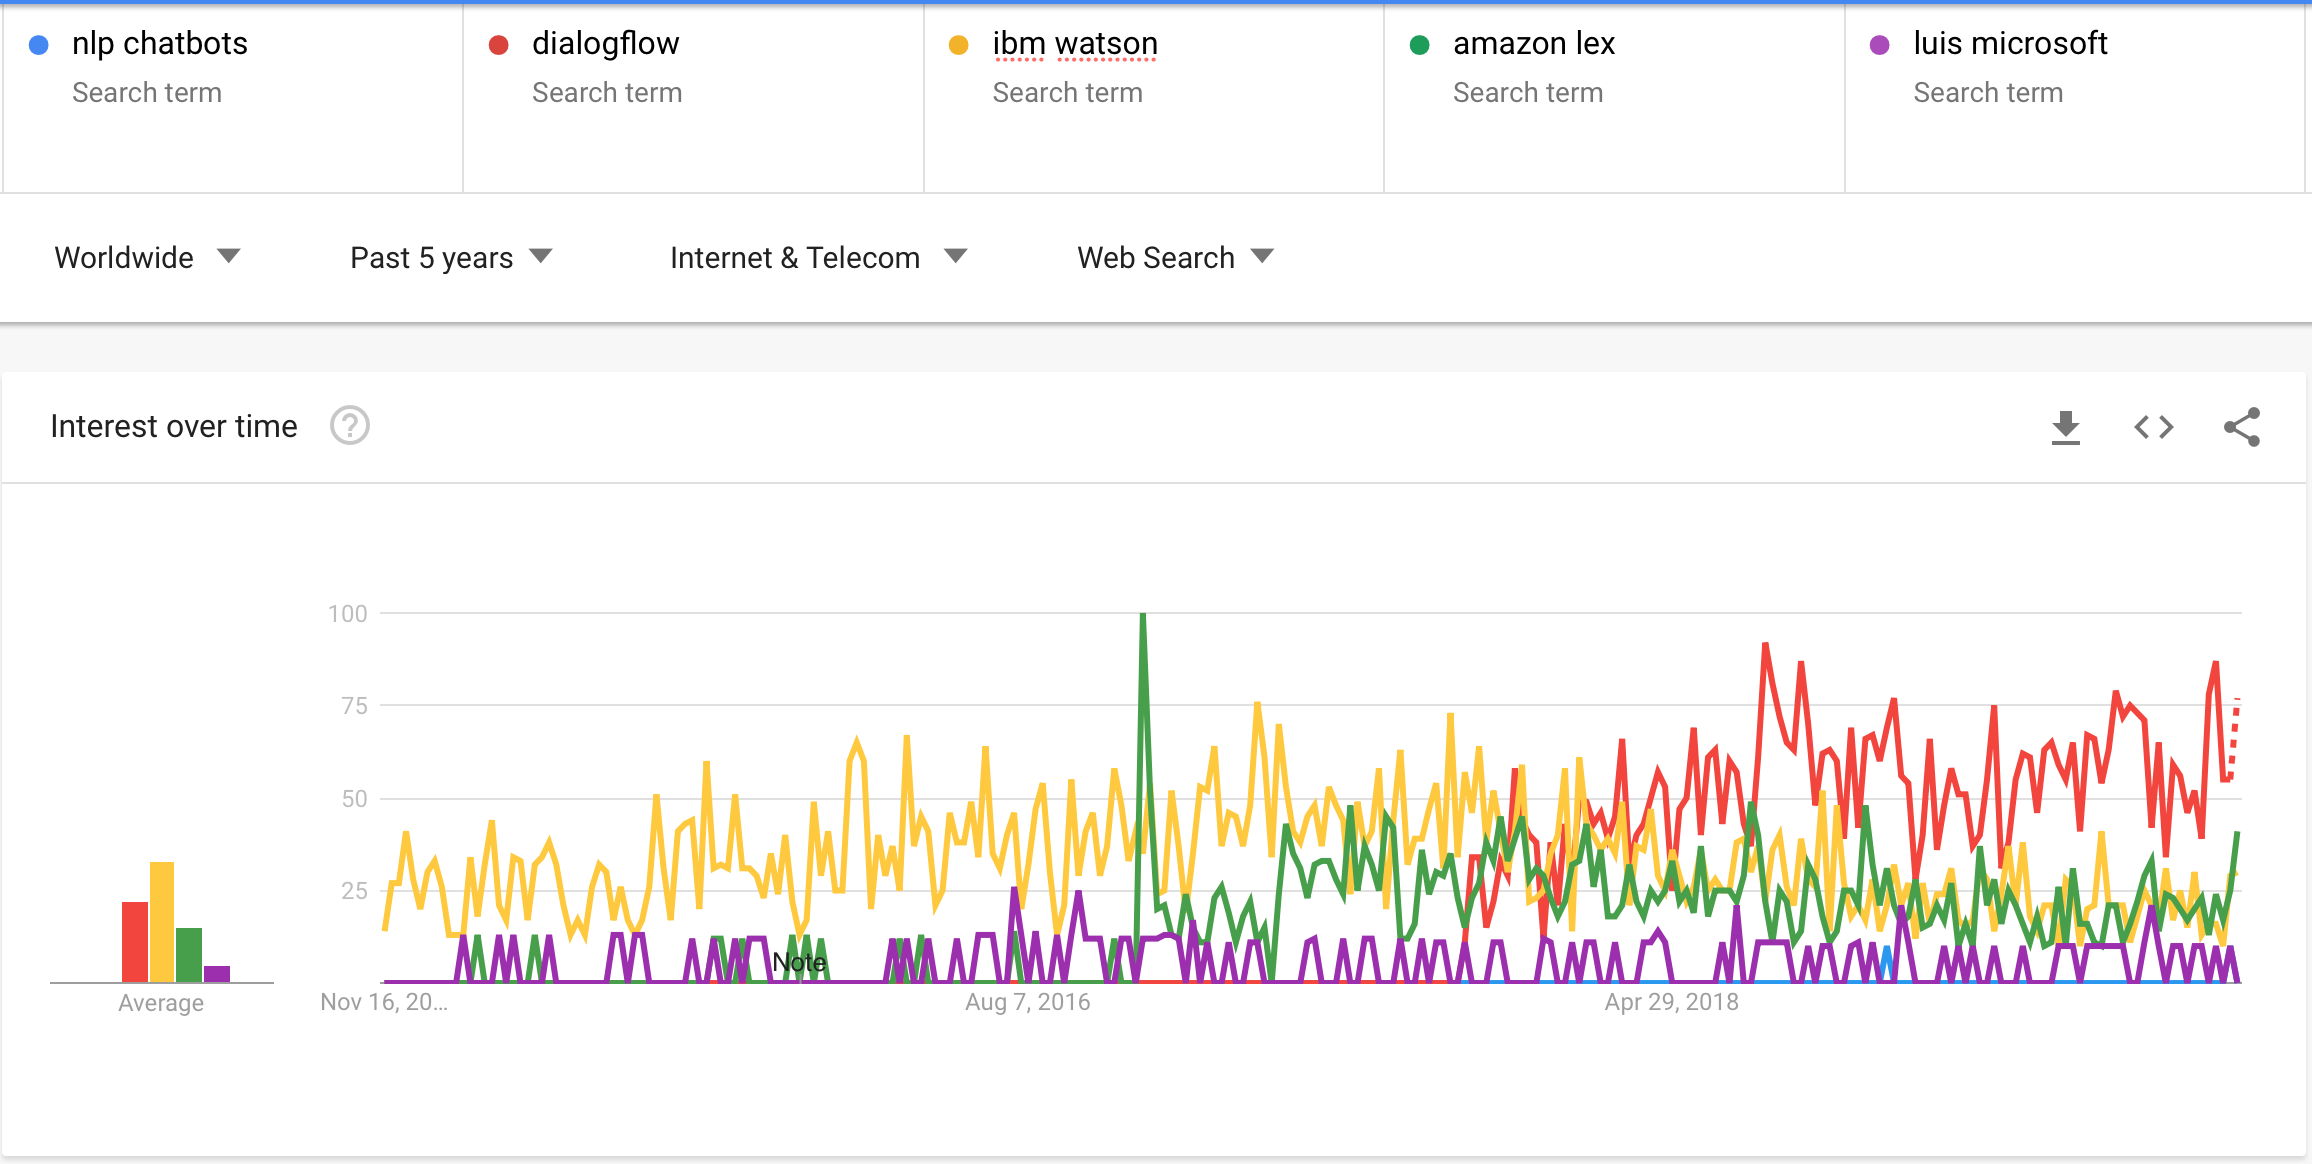
\includegraphics[scale=0.45]{MA-BA-Thesis/NLP_Chatbot_Comparison.png}
    \caption{Comparison of Google Trends for NLP Chatbots}
    \label{fig:nlp_chatbot_graph}
\end{figure}

This trend of growth among the different areas can be described in the figure \ref{fig:nlp_chatbot_graph} where we can see that there is an ongoing trend for DialogFlow over other chatbots despite the continuous big interest overtime in IBM's Watson.

\begin{itemize}
    \item Non-programming chatbots
    \item Conversation-Oriented chatbots 
    \item Platforms by tech giants' chatbots.
\end{itemize}
The breakdown of chatbots as described by Rahman\cite{chatbot_reference} describes a schema were bots are offered in different layers which include the tree based chatbots limited to answer questions and simple structures without getting into detail of the content. Then on a different layer the Conversation-Oriented chatbots use data as a foundation of information and Natural Language processing for further inspections.

In the Conversation-Oriented chatbot layer we can find that most clients have issues with training layers of data. Thus the biggest players in this category are the ones who handle and create models based on big amounts of data combined with entity and sentiment analysis. Furthermore, this leads us to the Platforms by tech gigants as described above which include DialogFlow which features pretrained models in combination with Entity and sentiment analysis which leads to ease of implementation and great gather of responses as well as context analysis.

\section{DialogFlow API}

In order to understand how the chatbot and the mappings is done its important to understand how the DialogFlow API works and what are the elements a usual chatbot looks upon before being able to convert and identify sentences into understandable machine context. To start we must understand that each sentence to be taken by the chatbot must used in two contexts, the first one to create an environment and the second to map the elements to entities in order to provide content for the chatbot to work on. To achieve this, DialogFlow uses Intents and Entitites as many other chatbots such as Rasa to extend the usability of the text recived. After the chatbot recives the text it will try to get mapped by using the trained entitites which are the words to be looked upon. For example in our case we would be looking for toolsets or problem definitions to map to unix tooling. Thus, our entities would be all the tools from the unix universe and the intent will try to comunicate the issue within this context. Additional entities can also be added and the more entities the richer the model will be. Mapping back to the example previously defined, we can say that within one intent, many entities can be mapped. To get ourselves in context we can say that the work of a text is broken into this area, despite that this will be further described in the development section to explicitly highlight the work of splitting and obtaining information from a string using a base test set.

Another important area from the DialogFlow API is the REST backend provided by google which allows us to talk back and forth with the google API to obtain the answers and also this will allow us to have structured responses since the back-end can handle JSON files. Also, the API features fulfilment which can allow us to reply using webhooks within a server app or even just to store and process a new answer using this API. Its worth mentioning that all the text will pass through the google API server. Moreover, there are additional features that will be explained during the development section that include how sentiment and entity extraction can be done in conjunction of the chat bot to further enhance the capabilities of the system. 

Finally, among the capabilities of the DialogFlow API we have composite entities and context which can aid the work of identifying subsections of entities and furthermore using the context to track a conversation within a set of responses using intents. This will be detailed in the development but is worth mentioning since most of the API is build upon this topics.

\section{Natural Language Understanding}
what Nartual language understanding is and why do we need it.

\chapter{Related Works}

There are several related works that train to aim to recreate or at least up to certain extent achieve a similar solution as the one proposed. In order to understand one of the closest paper in terms of content and approach we can have a look at Jacob's \cite{networkIntents} paper on Refining Network Intents for Self-Driving Networks which aims to use natural language to perform entity extraction and thus allow to create intents based on the extracted entities to perform certain operations. This is quite related to our work since it used DialogFlow as a basis as well and extended its usage with an intent mapper in order to allow users which have a median or low understanding of computer networking to use and create intents based on a relatively simple pipeline which allows to create entity extraction as a service.

The process described by Jacob uses google assistant to extract entities from the utterances and pre processes them into Nile. Nile is a intent translator that aims to try to gather entity information and map this to actual intents that can be performed by and android system. Once nile has completed the task this is later on passed on to the Intent Deployer who must deploy the service itself and finally deploy a network policy based on the previous intents. Throughout the process several important areas are described, for example the machine learning model which contains Nile as a decoder. Within this area, the encoder tries to identify the input entities which are then transfered through the Thought vector to the Decoder. The Decoder will aim to create an intent based on the extracted entities and output this to the intent creator.

The intent creator is out of the scope of out work, but is worth to be mentioned as it will gather the extracted entities into a new intent that will deploy policies. This can be done using the recommending system developed by Franco \cite{MENTOR}. Related to this work we can find other interesting mappers for NLP such as Cocoon which uses first-order logic instead of machine learning for creating the intents into configurations. Moreover Cocoon lacks the capability of a operator refinement and learning the operator intent over time which leaves it behind. 

In order to understand mapping of natural languages is good to have a look at Lumi, as described by Jacobs in Deploying Natural Language Intents with Lumi in \cite{networkIntents}. In this paper we have a glimpse into information extraction, intent assembly and deployment using a tool called Lumi which is in charge of handling all the resources and routing to the right scenarios. In this area there are several other aspects that must be taken into account for our implementation such as the intention aware detection and the entity extraction that also takes place in this tool.

\section{Rasa and NLU}

An important tool to take into account before understanding why we used DialogFlow as our preferred chatbot to take into implementation instead of Rasa an opensource ChatBot that with an open source foundation. Since Rasa features NLU Natural Language Understanding which For Chatbots look into 2 elements and whose work is to look into entity extraction which allows to map further resources into either an intent description or a further entity extraction. This elements are proven by Braun \cite{nlu_complete} and the extraction of this element is also shown to be the most efficient with LUIS \cite{nlu_complete} as it shows that the corpus of the entry text usually influences on the capability of the ML algorithm to fetch and extract successfully the entity from the corpus. Despite this, NLU focuses on mapping the entitites by default on chatbots but lacks the capability of mapping certain contexts and invalidate ambiguity within the context. For example, after the corpus is delivered then a further retrieval of another intent or a successful implementation must precede and thus query a common knowledge database in order to generate a message that could hold the main elements named:

\begin{itemize}
    \item Text Planning
    \item Sentence Planning
    \item Linguistic Realizer
\end{itemize}

This elements will allow to map the original query of the user, combined with the entity extraction to a generated response that could be capable of delivering further questions to gather enough entities to satisfy the context or end the query and reply with the current information. Furthermore, neither RASA nor LUIS proved to handle the entity extraction in a very efficient manner which denotes that more work is needed in the area to correctly address the issue of entity extraction and thus allowing the chatbot to perform a complete analysis.

\section{Chatbot Technology Challenges}

In a different area we are also presented some interesting aspects of how chatbots are still limited not only by context but also by the corpus in which they work and show that there is work related to context identification but clearly addresses issues with the p-values required to accept the proposed solution by Rahman \cite{chatbot_challenges} in which three different aspects are presented that must be taken into account to understand limitations of the current state of NLU and chatbot development that might cap our project or set a logical boundary. Rahman describes that the current challenges which still hold now a days are related to how we extract information for each query. 

They propose a theory which is used in most chatbots now a days, thus we use intents to map input to contexts and once this intent is recognized we can performs entity extraction to gather the important elements from the conversation leaving aside the facts that are not crucial for the implementation. In this way, the paper introduces B-Point Tree which outperforms the BST tree used in NLP Classifiers as supervised training which is the common technique used in chatbots. With this approach it is easier to infer the context and map the entities to the intents since you may have many intents to a single context.

\section{Network Tools that aim to help the SysAdmin}

Sula gathered information about protection services for a subset of types of attack and generated recommendations based on this. This relates to our work as it might contain several pieces of information that help us to extend our service past the gathering of requirements and delivery of information. In his work Sula gathered a table containing a set of services and a relative reference pricerange which could be used to map possible entity extraction outcomes to possible solution tools. The table from Sula \cite{recomendationSystem} gathered the following elements:


\begin{table}[h]
\centering
\caption{Services and Pricing from Sula \cite{recomendationSystem}}
\begin{tabularx}{\textwidth}{|l|l|l|l|}
\hline
Provider               & Service                         & Pricing                                    & Deployment              \\ 
\hline
Cloudflare             & Advanced DDoS Attack Protection & Free Trial                                 & Cloud based             \\ 
\hline
Imperva                & Incapsula                       & approx. \$3500 per month, \$5000 for setup & Cloud based             \\ 
\hline
Arbor Networks         & Arbor Cloud                     & on Request                                 & In Cloud \& On Premise  \\ 
\hline
Verisign               & DDoS Protection Service         & on Request                                 & Cloud Based             \\ 
\hline
Level 3 Communications & DDoS Mitigation                 & on Request                                 & In Cloud \& On Premise  \\ 
\hline
Corero                 & SmartWall Threat Defense System & approx. \$2500 per month, \$1000 for setup & In Cloud \& On Premise  \\ 
\hline
Flowmon                & DDoS Defender                   & Free Trial                                 & Cloud based             \\ 
\hline
Akamai                 & Kona Site Defender              & approx. \$6000 per month, \$3000 for setup & Cloud based             \\
\hline
\end{tabularx}
\end{table}

Here we can see a set of element that could be used to expand and use in our chatbot and can still can cause a beneficial impact on the system administrator experience. It is very important to mark that from this table not all elements are described in detail and not all solutions can be used to be mapped to all problems and thus there are underlying limitations.

Also, as it will be described later on many other services that also provide a comprehensive support system are available on the market and could be used to expand the usage of our chatbot.
\chapter{Approach}

\section{Extraction}
During the process of building the chatbot several steps had to be taken into account in order to generate stable data that could be used to expand and integrate with our desired chatbot. For this we decided to extract the elements from the Man Pages from linux in order to be able to generate a large amount of entities that could help us map each entity to a type of natural language element that will provide enough information to correlate the intent from natural language and the expected entities. To process this information we used a database that contained all the information regarding UNIX man-pages. The database we used for this is called Manned and was obtained from \cite{mannedDB} in order to extract elements from this database. The original schema from the database can be seen in Figure \ref{fig:manned_original} where it can be seen how a single index exists and for each element there are two partial sections which are the content or section for a Manpage and identifiers that can be queried to distinct if the element belongs or not to certain package. To expand this we can say that the database contains not only the recent elements but element from non official releases. In order to distinct and classify the information we must have classified and make some distinctions to be explained.

The database of Manned DB contains 18,926,291 manpages extracted from several organizations, this database weighted around 21 Gigabytes of data on a PostGreSQL Database and had the schema presented on Figure \ref{fig:manned_original}. This recopilation of information includes infomation from a few elements, to name them:
\begin{itemize}
    \item Packages
    \item Release Date
    \item Category
    \item Language
    \item Contains Section
    \item Architecture
    \item Section Arragement
\end{itemize}{}

Based on this we filtered the important information that could be used to train our chatbot.
\newline
\begin{figure}[h!]
    \centering
    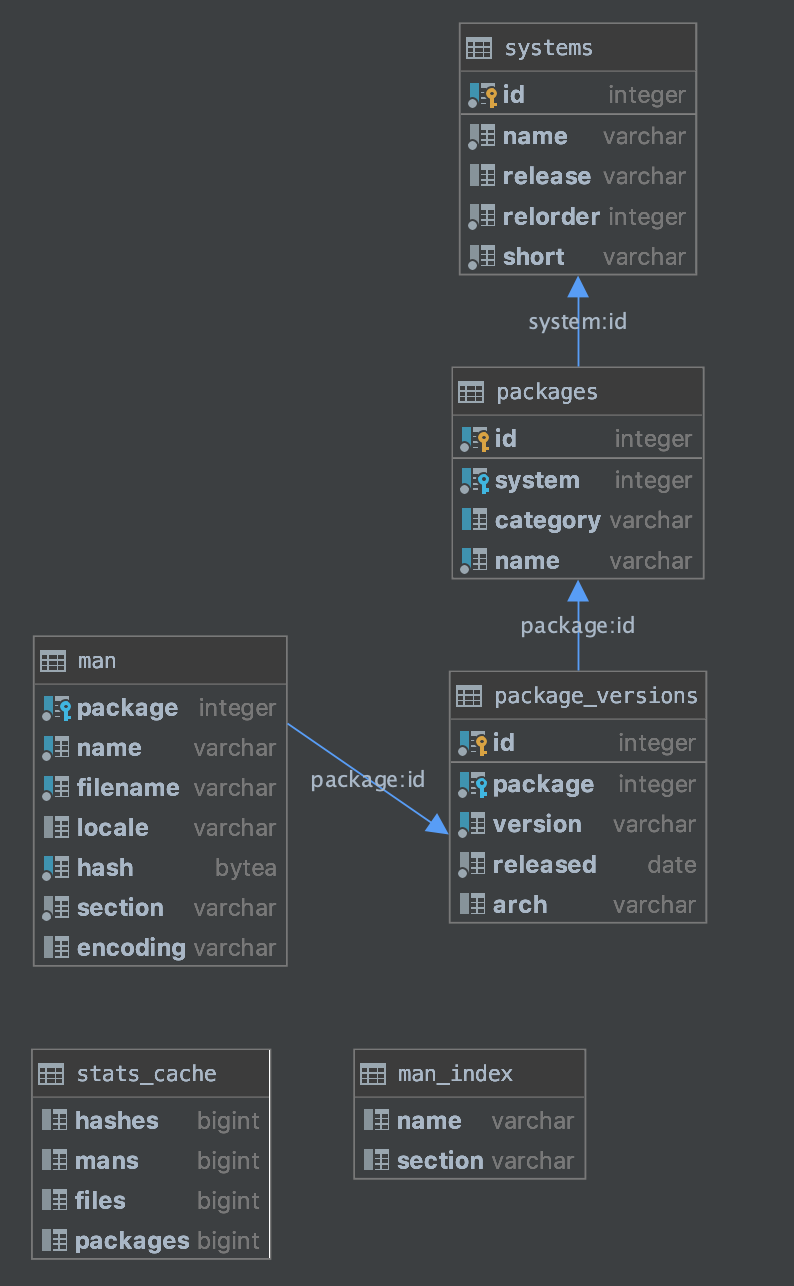
\includegraphics[scale=0.70]{OriginalDB.png}
    \caption{Database Schema from Manned DB}
    \label{fig:manned_original}
\end{figure}

\textbf{Package:}
To extract the right packages, the aim was to use the latest package from the current community edition. Meaning that for each manpage it must belong to a certain package such as Development or Community and so on and so forth, expanding this each package must be versioned with a single number. In order to extract the latest information in the most stable way we used the highest version number from the community edition. 

\textbf{Release Date:}
In order to obtain the most relevant information and avoid indexing information that could not be used only the latest version of a manpage was used. In fact, older versions could also be used and might have expanded the accuracy of the machine learning training phase but due to time constraints was not used. This will be further expanded on the Further Works section.

\textbf{Category:}
The categories can change from packages to packages and thus we decided to use the standard UNIX manpage as described in the Ubuntu repo, other packages contain a different set of categories and thus we decided to use the standard leaving behind the POSIX and d,e,f sections to follow a more standardized approach.

\textbf{Language:}
Despite the fact that DialogFlow can work with many languages and certainly most locales would've been beneficial for the project, to have a simple approach the proof of concept was developed aiming only for the English Language and thus, the other manpages that were not in English were discarded.

\textbf{Contained Sections:}
Is also important to mention that some packages do not fill the standard criteria for a manpage section. Most manpages follow a standard meaning that the must include:
\begin{itemize}
    \item name
    \item short name
    \item synopsis
    \item description
\end{itemize}{}

If the manpage did not include this parameters or they were not in the standard way then they were also discarded as mining the data would've been a difficult task that was not part of the initial hypothesis. What so ever, if we included them the algorithm should've been able to filter them as well.

\textbf{Architecture:}
Most servers run on a x86\_64 architecture also known as the AMD64 Architecture, thus we decided that filtering all manpages that were not built for this set of instructions would ease the job of processing the entities to the right parameters. Some tools that work only in the x86 architecture were also included as they haven't been ported fully to a x64 architecture but are still relevant for usage. So is the case of tools such as i386 tools such as WineHQ.

\section{Proposed Structure and Data Extraction}
Furthermore, in order to be able to work with this information we had to filter all the previously shown information using a rather simple criteria. To show how this criteria was generated a simple snippet of code is presented.

\begin{lstlisting}[language=SQL, frame=single, basicstyle=\small\ttfamily]
SELECT s AS sys, p AS pkg, v AS ver, m AS man
        FROM man m
        JOIN package_versions v ON v.id = m.package
        JOIN packages p ON p.id = v.package
        JOIN systems s ON s.id = p.system
        !W
    ), f_english AS(
      SELECT * FROM unfiltered
      WHERE NOT EXISTS
        (SELECT 1 FROM unfiltered 
        WHERE is_english_locale((man).locale)) 
        OR is_english_locale((man).locale)
    ), f_pkgver AS(
      SELECT * FROM f_english a 
      WHERE NOT EXISTS
        (SELECT 1 FROM f_english b 
        WHERE (a.ver).package = (b.ver).package 
        AND (a.ver).released < (b.ver).released)
    ), f_stdloc AS(
      SELECT * FROM f_pkgver WHERE NOT EXISTS
      (SELECT 1 FROM f_pkgver 
      WHERE is_standard_man_location((man).filename)) 
      OR is_standard_man_location((man).filename)
    ), f_secmatch AS(
      SELECT * FROM f_stdloc 
      WHERE NOT EXISTS
      (SELECT 1 FROM f_stdloc 
      WHERE (man).section = ?) 
      OR (man).section = ?
    ), f_arch AS(
      SELECT * FROM f_secmatch 
      WHERE NOT EXISTS
      (SELECT 1 FROM f_secmatch WHERE (sys).id = 1) 
      OR (sys).id = 1
    ), f_sysrel AS(
      SELECT * FROM f_arch a 
      WHERE NOT EXISTS
      (SELECT 1 FROM f_arch b 
      WHERE (a.sys).name = (b.sys).name 
      AND (a.sys).relorder < (b.sys).relorder)
    ), f_secorder AS(
      SELECT * FROM f_sysrel a 
      WHERE NOT EXISTS
      (SELECT 1 FROM f_sysrel b 
      WHERE (a.man).section > (b.man).section)
    ), f_pkgdate AS(
      SELECT * FROM f_secorder a 
      WHERE NOT EXISTS
      (SELECT 1 FROM f_secorder b 
      WHERE (a.ver).released < (b.ver).released)
    )
    SELECT (pkg).system, (pkg).category, (pkg).name AS package
    , (ver).version, (ver).released, (ver).id AS verid,
           (man).name, (man).section, (man).filename
           , (man).locale, encode((man).hash, 'hex') AS hash
     FROM f_pkgdate ORDER BY (man).hash LIMIT 1
\end{lstlisting}

Following the code presented above, the SQL query will extract the elements based on the criteria described in the previous subsections. This outcome was mapped within the same database before getting exported into the cloud. Figure \ref{fig:manned_edited} contains a diagram of the expanded database with the filtered elements into a new table.

\begin{figure}[!ht]
    \centering
    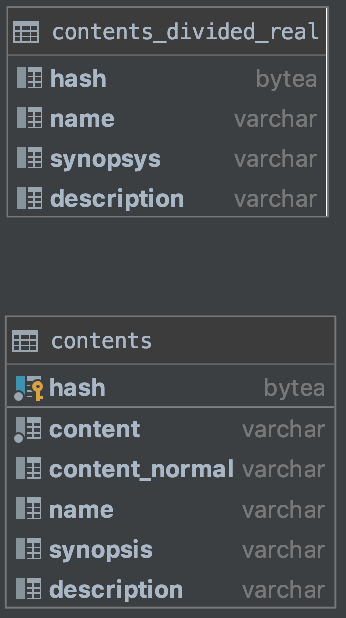
\includegraphics[scale=0.70]{MA-BA-Thesis/NewStructure.png}
    \caption{New Database tables from filtered data}
    \label{fig:manned_edited}
\end{figure}
They all contain 100221 entries that could be mapped into entities, in order to do this the tables where exported into a noSQL database that could interact with DialogFlow. In order to do this, we used Data Store by google which provides object storage within the cloud an allows dialog flow to extract and insert into entities as shown in figure \ref{fig:dataExtractedFlow}. To have a better idea of how all the components work in Dialogflow a graph is provided to expand and explain how the interaction was made faster for a big amount of data as described above.

The noSQL Database contains all elements sorted by keys which are then later on exported to the entity in DialogFlow using internal API calls. This was done by using a python script that took the relevant columns, parsed them and inserted them into the DialogFlow underlying layer. This script is provided in the Appendix and the logic works by processing chunks of information gathered from the database and converting them into data-frames that will be reinserted into the database while getting rid of the ROFF format \cite{roff}.

\begin{figure}[!ht]
    \centering
    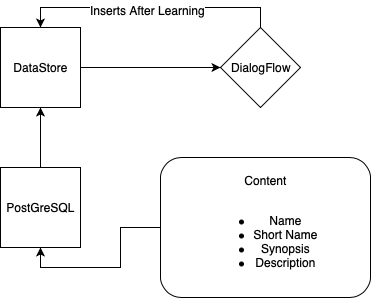
\includegraphics[scale=0.70]{MA-BA-Thesis/DataExtractedDial.png}
    \caption{Data Extraction and insertion Flow}
    \label{fig:dataExtractedFlow}
\end{figure}

The ROFF format is the standard for man pages but was extracted and removed using pre-processing headers within the python script. This allowed us to handle the information in a rather easy way so DialogFlow can consume it and use it. Despite this, the algorithm should be capable of handling or discarding files that are not formatted using the ROFF standard and thus discard the entities that are not matching the right setting.

\section{The DialogFlow Model}

In order to understand how the model is developed we must have a relatively clear understanding of how is that the underlying NLU model works under the hood. Even though this was explained in the Background Section is important to keep into account concepts such as Entities, Intents, Context and Composite Entities all these elements refer to Domain Classifiers, Intent Classifiers and Named Entity Recognizers as described by Su \cite{amazon_nlu}. In order to have clear picture of how each of this elements work together in the project is relevant to understand each element as separate. Thus, the underlying section of each one will be explain all together with a working description of the implementation of the intents in production.

\section{Intent}

The intents in DialogFlow are desribed also as Intent Classifiers (IC) within the NLU contexts and they recall the capability to identify certain mapped query based on a similar input query by filtering the elements existing in natural language and matching entities to the the ones from Entity Recognizers, this will be explained in detail in the Entity section. For starters there are two subsections of the Intent Classifiers as defined by Su \cite{amazon_nlu} in which we can argue between Supervised Learning and Pretrained Embeddings.

On the first hand, we can describe Supervised Learning which is what RASA is using we have to understand that the model works by classifier a query based on a model that is trained already. It works by training word embeddings and counts how often distinct words can be used as an input for the classifier. This is denoted in the paper by Wu \cite{amazon_space} where embeddings are trained from scratch using the n gram count algorithm. By the time the algorithm is trained we must try to use the input or original user query to match any of the relevant existing intents and thus identifying the original intent.

On the other hand, we have pretrained embeddings which is what DialogFlow uses to map or classify intents accordingly. In order to do this, each word is represented as an embedding and thus converted to a numeric vector. Therefore, we can find semantic and syntactic aspect of words in relation to other words that have a similar vector this is widely described in the word2vec paper from Mikolov \cite{word2vec} but the important findings regarding this paper rely within the fact that word embeddings can be used to relate words among each other using the following formula:
\newline
\newline
Bag of Words
\begin{equation}
Q = N \times D + D \times log_{2}(V).
\label{eq1}
\end{equation}
Skip-gram model
\begin{equation}
Q = C \times (D + D \times log_{2}(V)),
\end{equation}
\newline
As denoted by Mikolov where N is the previous words and V is the size of the vocabulary. Finally D is the corpus of the text. Also C is the calculated distance between the words.
\cite{word2vec}

Taking this into account, we can say that the process of intent recognition used by DialogFlow reassembles the one used by RASA and calculates the average from the input of the user to calculate distances using fastText embeddings and the desired model in our case gridsearch.

\begin{figure}[!ht]
    \centering
    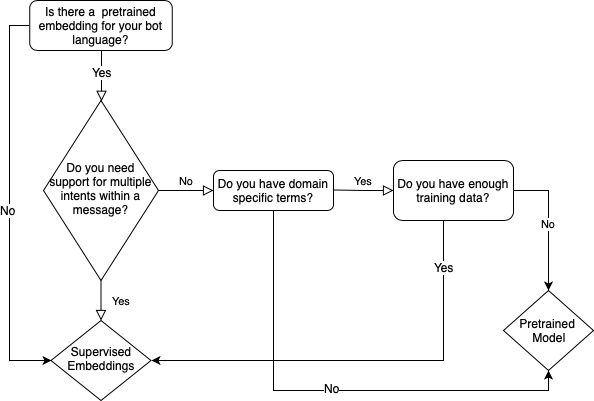
\includegraphics[scale=0.70]{MA-BA-Thesis/IntentDiagram.png}
    \caption{Diagram of selection for Pretrained embedding vs Supervised Training}
    \label{fig:diagramIntent}
\end{figure}

Using the figure \ref{fig:diagramIntent} we can reference that for our case using a pretrained embedding was the only option since we do not need to support multiple intents within a message and even though we do have specific terms for the domain the limitation in this case is the amount of training data available. Is possible that as the tool database grows and more intents are recorded and added as a future work a supervised embedding can be trained but this will be explained in the Further Works section. As of the models being used from Mikolov the CBOW referes to mapping words to a word based on the context so based on the user input we can determine if the input relates to an intent. Furthermore, we also have the Skip-gram model that works the other way around, mapping from a word a context; this is quite relevant as this will be used to gather and extract the right context from the input but this will be explained in the context section. It is also worth mentioning that our chatbot contains a set of intents aimed towards DDoS attacks since the proof of concept is targeted towards this concept. Keeping this in mind will allow us to understand that the intent base can grow to match intents from the Tooling extracted in the first steps but at the current state just a handfull of intents for tooling identification and analysis where left.

\section{Entity}

In each element of a sentence we must identify intents that will allow us to map the important elements within a sentence. Several examples can be provided such as "How is the weather today" or "Today we have good weather?" this two examples show how intents interact to provide the same set of information. For this case, the entities or important elements for further processing are Today as a time entity and weather as the requirement entity. Furthermore if we can identify this as a question then we would have successfully mapped the intent to the right set and thus would be allowed to expand this information to retrieve it from a third party service and provide an appropriate answer. 

In the case of our chatbot we would need to extract relevant information that would allow us to generate a file that could be useful for a recomender system to give solutions to current problems. Thus, we used elements from the extracted UNIX manpages to allow the ease of entity analysis and identification. To expand on this, the entities that exist or are added from the DialogFlow side are the ones obtained from the UNIX man pages and using the skip-gram algorithm on a pretrained model we aim to obtain embeddings that can map to the right intents. Also, this relies on the context that will be explained later on but on a first glimpse this is how the mapping between Entity and Intent happens in technical terms. Furthermore, we must expand on what an Entity is and how Entity Recognition works.

To understand entity extractors we must understand that there is not a single way to identify an entity but rather a set of choices. It is not known how Google handles the entity extraction but the scholar papers that recall entity extraction relate two main known ways which are:
\begin{itemize}
    \item Pretrained entity extractors
    \item Rule-based entity extraction
\end{itemize}{}
For each one of this there are specific tools developed and run diferent algorithms to support the extraction. spaCy uses a already defined set of pretrained entities which are generally known, its most likely to be used in DialogFlow as well and is the default method of identification in tools such as RASA. It works by using a pretrained model with a list of entities mapped to results and uses the same for entity identification. For our case this is relatively simple as we provide a list of entities that are meant to be identified. Thus, we can say that our method of entity identification reassembles the one of a pretrained model with transfer learning on top of this.

Also, Duckling allow us to create a set of rules to identify an entity similar to a regex expression but generally this was proven to under-perform spaCy. If we aim to have a very comprehensive entity extraction and identification we can combine all the existing methods to provide the best solution. 

\begin{figure}[!ht]
    \centering
    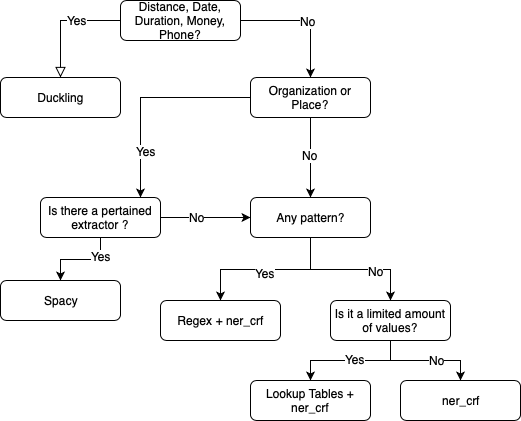
\includegraphics[scale=0.80]{MA-BA-Thesis/entity_extraction.png}
    \caption{Diagram of ideal entity extraction based on fallback}
    \label{fig:entityExtraction}
\end{figure}

The figure \ref{fig:entityExtraction} is presented by RASA and allows us to have a better understanding of how the chatbot entity identification fallback service works and which tool must be used for each case. Despite this, at the moment several tools are still being experimented with and DialogFlow provides only a beta feature for entity extraction but does not detail the underlying process also Name Entity Recognition (NER) is still on a develop stage and there are interesting approaches such as the one from Strubell \cite{NER} which explains the underlying structure of looking through a set of rules and uses aproximations on a pretrained model in order to get the best out of the model. Whatsoever, this shows that there is a trend to use pretrained models to solve the problem of entity identification as most entities can be identified from a preset entity and categorized model.

\section{Context}

The context of the conversation or Domain Classification relate to how an intent can pass extracted entities across other intents and use the extracted information to expand the conversation. This element is crucial in our chatbot since it allows us to use the previously obtained information to elicit or reiterate an intent in case there is no result that could be used to fulfill the requirements of the recommender systems. In order to understand how this works in DialogFlow we must get an understanding of how is that Domains get classified in upper layers and passed to other Domains or retained in a particular domain. Since two intents or more can live within one context and an intent might hold up for several contexts.

In order to understand how context manage and interact with intents it is important to clarify that the domain relies on information that must be passed among intents to hold a conversation. A good way to describe this lies within a normal context of a conversation where entities have to be extracted in order for the context to make sense. For example, if a george washington was born in the year 1732 and then as a followup intent we ask who was he, it is important to pass the main entity which is george washington to then next intent in order to be able to provide an answer using the current information. The time to live of a context is also relevant, thus if we want the information to persist over a span of intents then this must be defined too as an intent that contains too many entities could disrupt the results and the entities might overlap or the intent identification might fail.

Moreover, the elements that compose the identifier of a Domain Classifier are described by Jozefowicz \cite{domainclassifier} as classification in the neural networks domain and thus each element must go through a the network which yields a slow component. In practice our chatbot uses predefined domain identification, meaning that the intents map to which contexts but they context identification does not only rely on this but also on the IND and OOD utterance. To refine this, each intent maps which domain is recived and to which domain it must be addressed in order to avoid having the input domain overpowering the output domain in case of a multiple domain definition across multiple intents. In order to calculate which IND(in-domain) or ODD(out-domain) takes precedence Young-Bum came up with the following \cite{formulaDomainClassifier}.

To compute the utterance here represented by $\bar{h}$ we use a shared encoder and then the probability of the domain to be mapped must be defined using $\tilde{d}$ by mapping $\bar{h}$ to a $2$-dimensional vector for each domain $\tilde{d}$ as described by \cite{formulaDomainClassifier}
\begin{align*}
  z^{\tilde{d}} &= \sigma(W^{\tilde{d}} \cdot \bar{h} + b^{\tilde{d}})\\
  p(\tilde{d} | \bar{h}) &\propto
\begin{cases}
	\exp\paren{[z^{\tilde{d}}]_{IND}},& \text{if } \tilde{d} = d\\
    \exp\paren{[z*^{\tilde{d}}]_{OOD}},& \text{otherwise}
\end{cases}
\end{align*}
 where $[z^{\tilde{d}}]_{IND}$ and $[z^{\tilde{d}}]_{OOD}$ denote the values in the IND and OOD position of vector $z^{\tilde{d}}$.

Using this classifier we can exert and calculate the right utterance for each domain in a multi intent scenario taking into account the input and output context or domains. This behavior is represented both in RASA and thus in DialogFlow. In combination with both intents and entities this are the core elements of a query identification and information extraction for latter processing.

\section{Composite Entities}
As we previously defined in the Entity and Named Entity Recognition the entities are expanded from intents using different kinds of recognition through recurrent neural networks. In the case of composite entities which are entities expanded from the original entity. To refine this, an entity for example a T-Shirt or a Cardigan could possible and most likely have a color such as blue or white. Despite this, the refiner of the entity cannot exist if the entity itself is not present before. Following our previous example we cannot have a blue entity before defining to which entity it belongs. This allows us to classify easier the entities and gives us additional layers on the entity mapping thought this is only supported by DialogFlow and thus is one of the reasons that it was picked as the driver for the chatbot.

A sample of a composite entity is denoted in Figure \ref{fig:compositeEntity} where we can see how an entity is expended by using another entity which will use a skip-gram algorithm in the underlay architecture. The idea under this is that we are capable of defining granularities for our chatbot in case a user doesnt only want to give a detail related to an attack but also wants to specify with which degree of complexity it happened. Take the following example as reference:
\newline
"The web server is receiving high loads that reach 80\% of the total." 
\newline 
Hereby we can see that the entities to be extracted are mainly the high load and the server but as a composite entity the value of 80\% is relevant for attack identification and thus is added to the composite entity.

\begin{figure}[!ht]
    \centering
    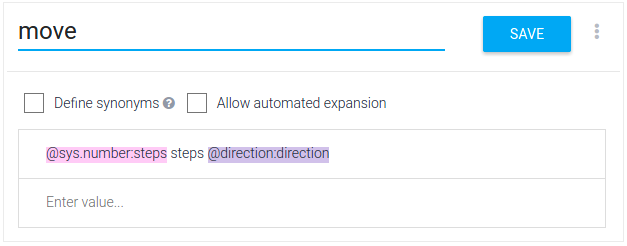
\includegraphics[scale=0.80]{MA-BA-Thesis/compositeEntity.png}
    \caption{Composite Entity as entered in the DialogFlow UI}
    \label{fig:compositeEntity}
\end{figure}

\section{Entity Definition for DDoS}
Among the most relevant elements of the chatbot lie the entities which are meant to be mapped in the intents, thus they had to be extracted and inserted. For our case we researched into the most common entities to be extracted when a network administrator was under attack by a DDoS attack and thus we came up with the entity based table \ref{tab:DDoS_entity}.

\begin{table}[h!]
\resizebox{\textwidth}{!}{%
\begin{tabular}{|l|l|}
\hline
denial of service & denial of service, dos \\ \hline
High number of request & High number of requests, High load, accumulated load, high request number \\ \hline
UDP Flood & UDP Flood, UDP Packet Attack, UDP Packet, UDP \\ \hline
ICMP Flood & ICMP Flood, ICMP packets, single packet, ICMP echo, ICMP echo relay, ICMP replay \\ \hline
SYN Flood & SYN Flood, SYN packets, SYN attack, SYN requests \\ \hline
Ping of Death & Ping of Death, POD, PoD, Denial Ping \\ \hline
Smurf Attack & Smurf Attack, smurf ping, smurf request, smurf \\ \hline
Fragmented Packet & Fragmented Packet, fragmented request, fragmented information, partial packets, partial requests \\ \hline
Low Resources & Low Resources, low available resources, low amount of cpu, low ram, low disk \\ \hline
overflow spoof & overflow spoof, overflow spoof packet, overflow, network overflow \\ \hline
unresponsiveness & unresponsiveness, unresponsive, takes too much time, slow, froze, not responding, not responsive \\ \hline
\end{tabular}%
}
\caption{Denial of Service Entity Identification}
\label{tab:DDoS_entity}
\end{table}
It is important to mention that the elements that were added for the definition of the DDoS table are coma separated values denoted by several elements on the second column which map to a single identifier on the first. All these entities can be expanded to match a large amount of identifiable elements that are present in an ideal DDoS attack and thus create a generalized solution. In our case we based the table on the work from Chen \cite{ddosAttacks} which described some of the basic attack elements in DDoS related issues and used them for identifying vectors. Also, the elements can be expanded and used in combination with composite entities such as numeric values and distinct identifiers. For example, if a server is receiving a fragmented packets and the network admin wants to describe how many fragmented packets are being received this is a possibility that could help create a solution or even distinguish a DDoS attack from another kind of attack.

Although, this is only a partial part of the whole setting that can be found in the code of the chatbot which expands the entity extraction with other elements such as victims of the attack which can range from single units to multiple vectors are can be required in combination with the described base entities. Moreover, at least this two elements, victim and attack vector are required. Depending on the granularity of the chatbot more entities might be required and mapped to fulfill the needs of the recommending systems. This will be described as well since the model relies on the current status of recommender systems, for our proof of concept the work was based to fit a general model and in detail with MENTOR \cite{MENTOR} and thus the elements that are present at the time are meant to match the ones from the recommender system.

Furthermore, DialogFlow features fuzzy matching and syntax analysis meaning that if a user inputs a result that is close enough to the intent the NER will match a good approximation to the entity. This can be further tweaked but for our chatbot we enabled the fuzzy chat to enable input and testing in cases of results that closely reassemble the original entity such as "ICMP and icmp" or "fragmnted packet" and "fragmented packet".

Moreover, it is also important to list some of the other entities that were used in the chatbot such as the types\_problem which allow us to pick the right elements or attack vector whether we are seeing an attack or we are looking to information from an error. To expand how the Entities relate to each other we can use Figure \ref{fig:EntityRelation} were we can see that there is a relationship among most entities that would allow us to extract the information in a cascade manner, thus if one element is obtained or present then the following elements would be desirable but this heavily relies on the needs from the recommender system. Also its worth mentioning that the intents that use this could map to one or more entities so this should not be the limitant in our case.  

\begin{figure}[!ht]
    \centering
    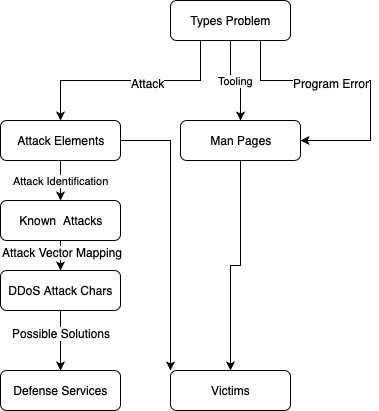
\includegraphics[scale=0.80]{MA-BA-Thesis/EntityRelation.png}
    \caption{How the existing relations work in the entity tables within the DialogFlow API}
    \label{fig:EntityRelation}
\end{figure}


Each element of the entities expands to a set or subset of similar entities which are matched by using fuzzy matching. Regardless, there are several ways in which we can expand the existing entities by using a similarity dictionary to increase the amount of similar entities to match the NER. Whatsoever, we did not proceed with this method in our case due to the precision needed for each intent and the non standardized way to calculate a vector based on its context. Using a skip-gram method could have given us a good amount of material but due to the hard process of computing nearest neighbors in the attack context, the results could have ended being to skewed to be used by the DialogFlow model. Also, some elements presented are not in use, for example in figure \ref{fig:EntityRelation} the Defense Services are not being mapped but this will be later explained in the next section. Is important to say that most entities were optimized to aim for DDoS detection as this was the proof of concept of this work.

\section{Creating the Intent Map and Training Phrases}
The Intents are made to map all the user input into the right entities, for our original idea to take place we came up with several possible intents to map into tools to aid the user and set a low or high level of granularity depending on the expertise of the user. Whatsoever, we realized that mapping a large amount of entities would require a relatively large amount of intents and thus to provide a proof of concept this was no feasible. In the light of this, we decided to aim for specific use cases such as attacks and to get into details into the DDoS attack which is a very well known and detailed type of the attack within the cybersecurity area. It is worth mentioning that throughout the setup many cases where implemented and many intents could possibly overlap others, thus we do not only have intents aimed towards the DDoS scenario but also the default ones for tool assessment. Nonetheless, all these intents must be mapped into the right solution and thus we will only expand into the ones aimed for DDoS identification for ease of use and to have a deterministic point of view. Also, all the test cases will be performed taking this into account and the chatbot is optimized to work under these settings as a proof of concept. Therefore, even though this set of intents was created for the mentioned attack the basis would be the same as it will be described later on for all other types of attack.

An intent in DialogFlow is composed of several elements that allow us to increase the probability rate of a right intent classification. Within the Intent of DialogFlow API we must define several elements that will aid us to help or expand the granularity accordingly.

\begin{itemize}
    \item Contexts
    \item Events
    \item Training Phrases
    \item Action and parameters
    \item Responses
    \item Fulfillment
\end{itemize}{}

All the elements that belong to the list above are part of the intent and a correct definition of each will allow us and expand the user experience and the accuracy rate depending on the right settings. We will describe them in detail and each element will shed light on why its dependent for the complete use of the entity, thus elements such as Contexts or Training Phrases should not be strange at this point but will be detailed so there is a high level of understanding. It's also important to mention that to set up the granularity of our Chatbot correctly several intents are needed, we wont get into details with this but it is important to mention that not all intents will define the same granularity and thus having multiple intents for multiple contexts is acceptable in the way that otherwise it would be hard to come up with different intents for the same granularity, thus intents map to different contexts depending on the granularity selected by each intent.

\subsection{Contexts within Intents}
Whenever we must define an intent this must belong to a context and the context will parse and pass all the elements among the intents so they can be further used. To understand this as explained in the domains we must pick to which element it must go into and out of, this also can help to set for how many intents we should keep the context. This is generally used to keep track of the right information across intents and specially useful if you have more than one parallel or similar intents. Something important to take into account is to prevent overwriting the information extracted by an entity in the context, since a context such as george washington can be passed across the whats the age intent but it can also get overriten by another NER such as abraham lincoln and thus pass the context of george washington but overwriting some elements but not all. In order to prevent this our chatbot focuses on single contexts and unless is quite necessary has a relatively short time to live on the context across intents such as 1 or 2 intents as a maximum. In order to describe this, we can picture a set of intents that relate to each other through the extracted entities but communicate using contexts with a short time to live.

\begin{figure}[!ht]
    \centering
    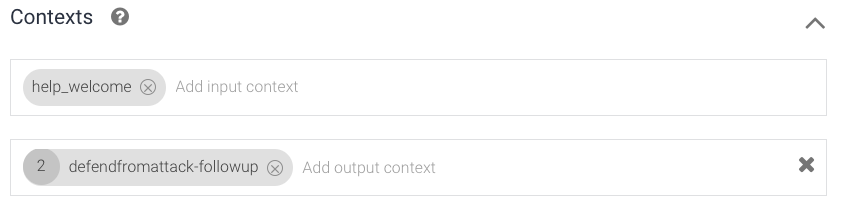
\includegraphics[scale=0.65]{MA-BA-Thesis/Contextsdemo.png}
    \caption{Demo of how a context interface looks like and the in and out contexts from the domain.}
    \label{fig:contextDemo}
\end{figure}

As shown in Figure \ref{fig:contextDemo} the number of time to live must be defined in advance and is possible to have multiple input contexts and also multiple output contexts. The benefit of this is that another intent is matching the classifier it will also pass the context is it matches the input context increasing the rate of accuracy of the intent classifier. Therefore, we set up a set of contexts within the intent dialogflow that relate to the following:

\begin{itemize}
    \item Welcome Context
    \item Identify Issue (Attack, Tool, Error)
    \item Map Attack
    \item Gather Attack elements
    \item Iterate over attack elements
    \item Goodbye/ Parsing
\end{itemize}{}

This are the default contexts used to get the information through each set of intents, and for each one there is at least one or more intents matching either in the input or output.
\subsection{Events}
Events are meant to take place whenever there is a desired action without being mapped by an intent. For example, if we decide to extend the usability of our chatbot past the UI and we want to trigger an intent based on an event such as location and thus ask a question or query for an intent just in case of this event or trigger happening. There is room for improvement here, as its possible to use this feature to automate the process of solution finding based on standardized problems such as Fragmented Packet Count above certain percentage and thus launch intent to query for current web status from the user and based on this information create a solution that could aid the network administrator to ease the problem even before the user asks the chatbot for help.

The current status of the chatbot does not allow us to expand on this but will be further discussed in the Further Works section.
\subsection{Training Phrases}

Perhaps the most important part of the chatbot and a remarkable part of the research takes place in the Training Phrases for the intents in the chatbot, since without them is hard to come up with a feasible solution that would approximate to the right entities. Based on this training phrases and the NER classifier the intents get mapped and identify entities, thus providing the right set of queries is important and can ease the job of a Fallback event.

The underlying work of providing training phrases aims to have enough information in the intent classifiers in order to assess if the loss function has to correct and assert in a better way or if the result was accurate enough. For the intent training we must provide positive examples or examples that reassemble the original query or that are acceptable enough. Since the process takes place in a higher layer of a pre trained model there is no need for negative examples in this case, whatsoever it is important to take into account that fallback intents which are queries whenever there is no apparent result from an intent usually mapped from a context and those are trained using negative examples or the opposite of what the intent should be. The underlying concept creates another classifier for intents to expand the basic classifier with elopements that could be considered unusual. Despite this, all classifiers calculate the accuracy of an intent in order to match it to the best intent and if certain threshold is not reached then it will try with the fallback intents. Similarly, we have default intents that will match an expected response and can be automatically generated such as Yes, No, Later, Cancel, More, Next, Repeat and so on.  This allow us to generate intents for simple responses within the conversation and through a series of tweaking we aimed to the best interaction from system administrator to reach a DDoS attack scenario which by itself is rather complex.

It is also important to mention that the training phrases must reassemble a close interpretation of the real query by the user but should not necessarily be equivalent since there must enough range of similarity for a proper classification, meaning that between training phrases there must be enough space for the real queries. Also, we could further process the successful queries obtained by the users and reinsert them into DialogFlow to latter use them as training phrases to aim for a constant improvement.

\begin{figure}[!ht]
    \centering
    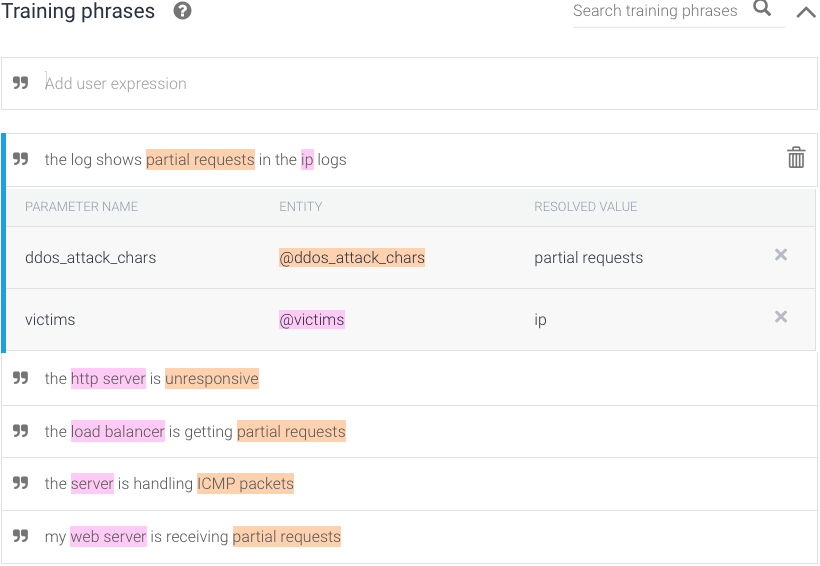
\includegraphics[scale=0.60]{MA-BA-Thesis/trainingPhrases.png}
    \caption{Example of training phrases with identified entities prior to training and resolved values}
    \label{fig:trainingPhrases}
\end{figure}
As shown in Figure \ref{fig:trainingPhrases} we can see that the training queries must reassemble to the real query but should not be contained. Also, it is important to mark down the entities to help the NER to identify the entities within the context. Most of them are resolved automatically after a few training phrases are entered meaning that you could already have an approximation of how are the entities getting resolved by the previously entered entities.

Is also worth mentioning that the parameter value represents the bucket or bin in which the entity fits, thus it behaves rather like a category which is also parsed in the generated JSON file. The resolved value is the actual value which holds the value for the element, as mentioned before an intent can have several entities of the same type within a single query.

\subsection{Action and Parameters}
Another important part of the chatbot interaction is the actions and parameters to be performed. The action can allow us to send an identifier through the intent that will hit Fulfillment and allow us to move the response or gather information with this identifier. Also, this action can trigger certain activities by Google such as turn on lights or similar but must be expanded into how the work applies to each element. In our case we decided not to use any action within the chatbot since the UI only requires a simple conversation without too much content and does not feature location or any additional service that could be provided through the google API.

Then on the parameters side it is important to specify which entities we aim to gather and which ones should be present in order to have a successful intent, this particular area is very important since the outcome of the intent might not be successful and hence instead of having a fallback intent to redirect to the original intent we aim to use a prompt within the intent to specify a question that guarantees that the entity will be gathered and thus mark the intent as complete. Once again, once this happens the response is passed to the Fulfillment engine and then shown in the UI. Even though we must define the parameters so the chatbot can know what to look for, not all of them are required and thus the prompting will only happen if the entity is marked as required. Furthermore, we can also ask for a list of values meaning that you could describe a set of symptoms of attack vectors to be parsed and if one or more are missing then they could be prompted. Likewise, all the elements as a list will get parsed and tried to match with composite entities in case this is available.

Since the prompt is our intent within the intent we can use elements from the context to guarantee or rise the possibility of the desired entity to be gathered. Within the prompt we can use elements that were already extracted for the intent, for example we could extract the values server load but if the kind of attack was not explicitly mentioned then we could make a prompt similar to this:

"Please provide the symptoms that the server was experiencing during the load"

And thus passing the already extracted entities to ask for an accurate answer. In order to be able to bypass or score higher in the Turing test, the chatbot features a set of prompts meaning that it will not ask the same question twice to simulate the conversation with a human or simply to try to ask the same question in a different way so is more likely that the right entity will be obtained from the input of the user. Whatsoever, since we just require a handful of intents to be able to match MENTOR not to many prompts were defined but could possibly be expanded according to the needs of the model. Also, the parameters can be reused within the intent meaning that if at least one parameter was identified it could be used to gather other similar parameters. Meaning that for example if the web server is under ping of death requests, we could also ask if any other device is suffering from a ping of death request directly to the user if the NER identifies the entity successfully.

\subsection{Responses}
In order to make the chatbot dynamic and enable a good set of interactions providing more that one response is always desired, these responses can go from very simple responses using the extracted information from the original user queries or even more dynamic including custom content to expand the user experience. Usually the message flow travels across fulfillment which will be described later on. Under the hood, the message from the user gets extracted and then sent to the DialogFlow Engine which runs the previously described algorithms to obtain the intent classification, the entity name and maps to the right context or domain. After this steps, the message can be sent if decided to fulfillment which will preprocess the message using JavaScript ES6 code. This can be used to expand how a response gets mapped to the user and which elements are used in the response. For example, we could obtain the information about the DDoS attack and based on the type of attack lookup in the database for solutions that could match this and provide a real time response using fulfillment. In this case the recomender system would not be needed anymore and thus for our chatbot the Dynamic responses are not used but in practice we could provide code, images, audio and so on and so forth to enrich the response from the chatbot. If required we could also send locations or elements related to the Google API stack of applications.

The answers can also be sent through other already integrated services that do not belong to the Google Stack API such as whats-app or slack, giving our chatbot a wider range of opportunities to interact and expand the usability with teams or even pre programmed bots. Also, it's worth to mention that we can mark the end of a conversation within the response and this will flag the intent as the last one triggering a final response and our chatbot will use this flag to create an array that will be parsed into a JSON which can be fed to the MENTOR system to create an accurate solution. As a further work in this aspect we could possibly wait for the answer from MENTOR and using the output we could modify the answer and provide an answer in realtime for the network administrator. Moreover, we can also submit multiple responses of an intent meaning that not only one channel can be used to answer for example if we manage to identify the issue we could possibly forward the solution using another channel such as slack or a call to an endpoint to implement the solution provided.

\subsection{Fulfillment}
The Fulfillment aspect of an intent is one of the most interesting areas of the chatbot since here we can manipulate the data as it reaches the server and thus we contain both the information from the API and the processed information from the machine learning algorithm. Thus the fulfilment allow us to extend the existing functions using customized code, most of it can be expanded into real functions using an external micro service. A good example of this could be shown in Figure \ref{fig:cloudFunction} where we can see that through Fulfillment we can connect to the cloud functions provided by Firebase and also the database containing all the tooling information extracted from the manpages which is stored in datastore as objects.

\begin{figure}[!h]
    \centering
    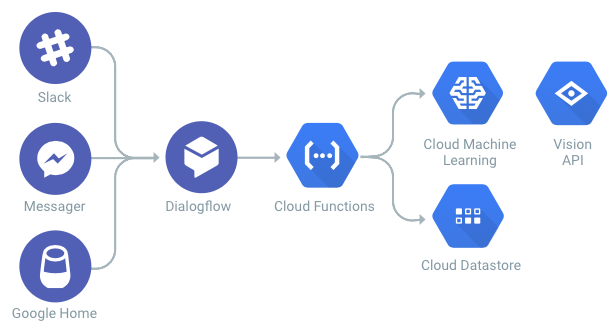
\includegraphics[scale=0.60]{MA-BA-Thesis/cloudFunctions.png}
    \caption{Map of how DialogFlow can interact with cloud functions to expand functionality of the results}
    \label{fig:cloudFunction}
\end{figure}

At the moment the chatbot uses the fulfillment in some important intents to fetch relevant information and to help to build the JSON tree and storing the built information external of the contexts and thus persisting the information. To expand this concept we can see that the elements obtained through a simple subset of requests is shown in Figure \ref{fig:responseArray} where elements are filtered already such as the classification score or the amount of intents required to reach the stage. All these are filtered using the fullfilment and since the fullfilment integration uses datastore is also possible to use elements obtained from there for further expansion of the response. Since the method control for fulfillment is enabled we could use other machine learning algorithm to further train our responses or to even generate a solution to have a solution independent of the recomending system.

\begin{figure}[!h]
    \centering
    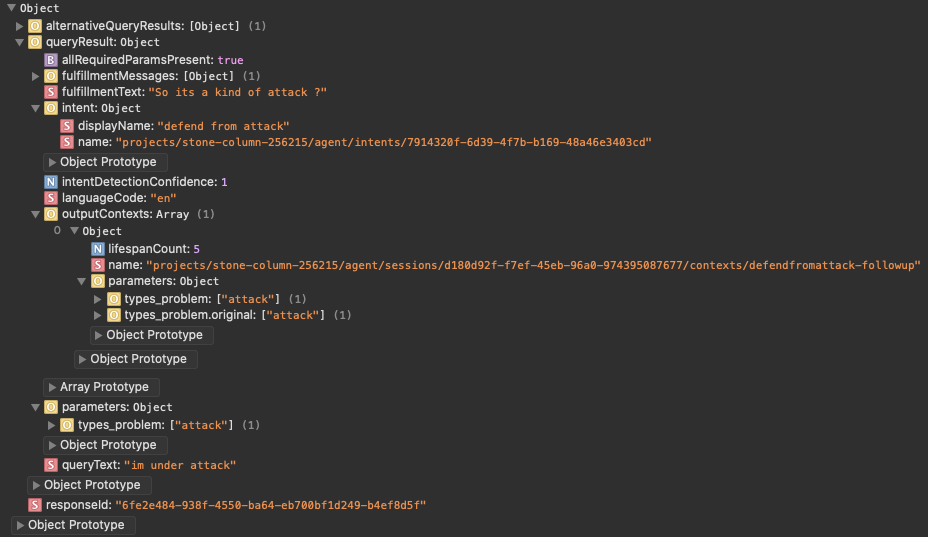
\includegraphics[scale=0.50]{MA-BA-Thesis/responseElements.png}
    \caption{Elements that are contained after processing an intent in fulfillment in DialogFlow, extracted from the UI}
    \label{fig:responseArray}
\end{figure}


\subsection{Overall Implementation}

All the elements have to be used in conjunction in order to generate a set of intents that can interact with other intents and fetch the information throughout the process. In order to achieve this we must define which entities are to be extracted in order to fullfill the goal of generating a JSON file that can be fed to MENTOR \cite{MENTOR} to generate a solution for the system by using the external services that can guarantee defense against attacks. To see how is that they interact with each other the diagram from Figure \ref{fig:intentFlow} describes how is that the components interact with each other to fulfill either goal. Is worth to mention that despite the amount of intents these have to be created in a unique manner and thus are limited by the amount of intents we want to create. For our proof of concept we limit ourselves to the flowchart from Figure \ref{fig:intentFlow} but it is important to mention that we must go through this procedure since an important element of NLU is the fact that we want to understand what the language means rather than what it is per se.

Each element correlates, for our aiming round we take into account the hello intent which will make sure that there is a human validator. Later on, we have the attack identifier which will aim to identify if the users suffers from an attack, a problem with an application or is looking for help with a tool. In our case we will only aim to fulfill the attack path. Once the attack is identified which could also be spread as a set of entities and symptoms to match to a right kind of attack but for now we will try to aim for DDoS attacks which have rather common symptoms. Once this is done, the user could input large sets of intents to match as long as there is a victim and a symptom or a set of symptoms which are also referred to as attack vectors. At some point all the details about the attack will be described and fetched to this intent, thus will pass on to the MENTOR \cite{MENTOR} funnel. In this funnel we will aim to extract all the key elements to create a recommendation through mentor. To list the elements are:

\begin{itemize}
    \item Type of Service : If the service requested is active or passive (Right now or to prevent later on)
    
    \item Type of Attack: Details about the Attack (Gathered by the attack vector intent)
    
    \item Region: Defense systems and deployments are available per region, thus this must be provided
    
    \item Deployment Time: How much time is available to implement the solution (Larger solutions are better but take more time)
    
    \item Leasing Period: The period for which the service must be contracted for at least.
    
    \item Budget: The budget for providing the service that will guarantee a defense.
\end{itemize}

With all these elements into account we can start to describe the funnel and which elements are mapped to which intents. This is a very important part of the chatbot as without it is impossible to generate results that have a good amount of content for the recommending system to work. Is also notable that if at some point we do not want to fit the recommendation from mentor we can type 'End here' or 'Finish here' which will terminate the event with the parameters handled up to the time. It is also important to say that from the gathered elements the intents can be triggered based on the input context thus the mapper or vector element attack identified can be queried from several points of the conversation just to guarantee that no data is lost due to missing the context of the conversation.

\begin{figure}[!ht]
    \centering
    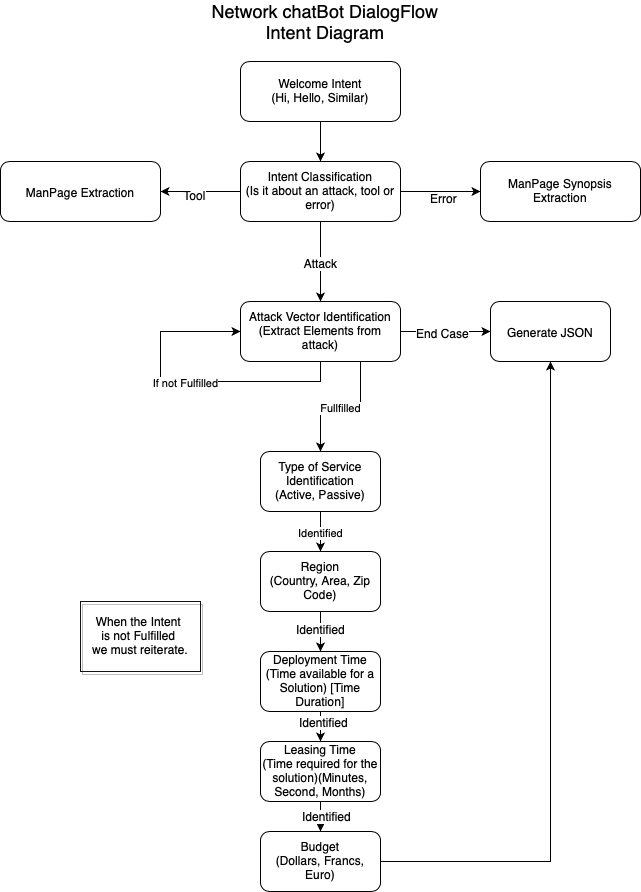
\includegraphics[scale=0.60]{MA-BA-Thesis/IntentFlow.png}
    \caption{Intent Classifier Flow to map elements through the DialogFlow API. All the Contexts are excluded from this graph as they are described in the context section.}
    \label{fig:intentFlow}
\end{figure}

To be extended.

\chapter{Prototype and Implementation}
\section{UI and Usage}
The application was designed using Javascript and a React Framework in order to allow hotswap and component structures that can expand the usage even further. For This purpose we used a simple stack with a pipeline. The underlying idea relates to how to query the intents from the user and at the same time build a stable pipeline that will allow an easy development using tools that are available online. For this the backend of the react client uses Heroku for the the deployment stack, meaning that the set runs under an automatic deployment handled by Heroku on the client side of the application. Thus a Git Repository was created to map all the elements and trigger builds made from the repository. Thus we would have the heroku backend pulling from the git repository and launching the app in an updated manner since it uses the latest commits to automate the deployment.

The application itself does not feature many functions besides obtaining queries as input streams from the user and filtering or cleaning the information prior to be sent to the DialogFlow API. Once the information is received by the API then Fulfillment will gather all necessary elements and refine the information that must be returned to the client. Once the client receives the information then it is stored in the session Storage of the browser where we parse elements such as the identified entity and the entity bucket. It's important to mention that the bucket where the entities are stored could have different granularity and thus are likely 
to differ from implementation. In our case to handle a proof of concept we aimed to have a standard implementation aiming to a standard attack under this concept. Whatsoever, once this elements are saved in the client we can manipulate the answer to be shown to the user but the desired behavior will log the result and keep adding elements over a custom array. 

One important aspect of the application is that in order to communicate with the API of DialogFlow it must use custom keys that are only available using the framework provided by google. In our case google had issues switching from the API v1 to v2 and thus we had to hard code the used keys and create a custom login screen that would allow us to interact with the server directly without a server side client. Thus there is an extra class that is outside of the scope of the initial functionality of the application that is used for this. Moreover, the functionality of the forms do not rely on an external framework besides react. This will allow us to have a interactive web form that can be used with almost any device, to show the interaction the following screenshots of usage are shown.


\begin{figure}[!h]
    \centering
    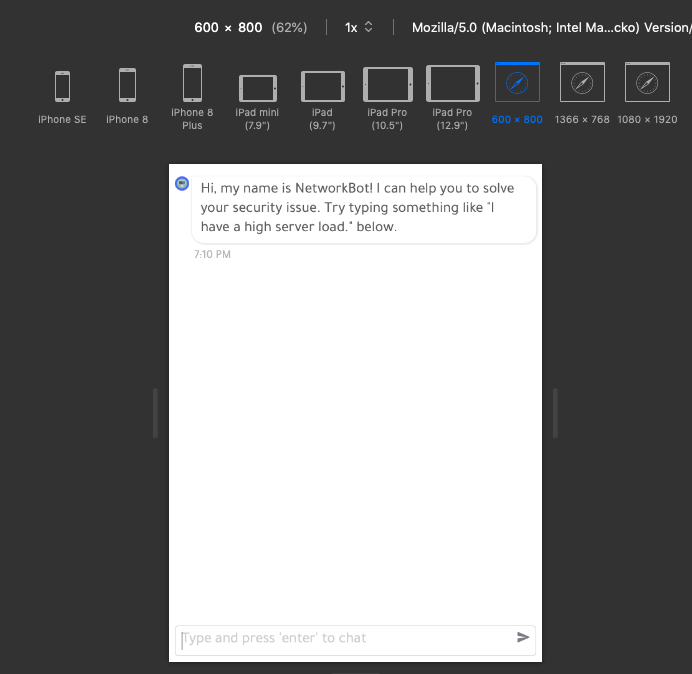
\includegraphics[scale=0.65]{MA-BA-Thesis/webUIScreen.png}
    \caption{Web User interface for the Network Chatbot}
    \label{fig:screenWeb}
\end{figure}


\begin{figure}[!h]
    \centering
    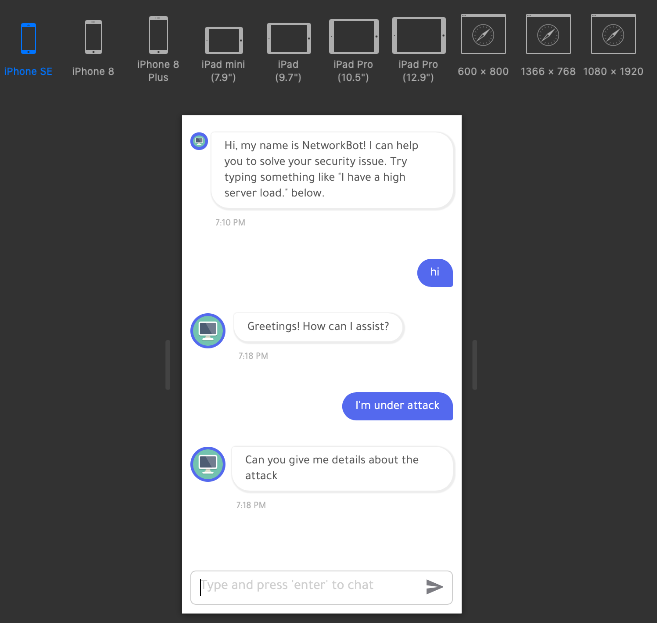
\includegraphics[scale=0.65]{MA-BA-Thesis/iphoneScreenUI.png}
    \caption{Responsive web interface as seen from an Apple iPhone 8.}
    \label{fig:screenIphone}
\end{figure}
 As seen in Figure \ref{fig:screenWeb} the react form scales according to the client need yielding a webclient that is reactive and has a relatively low page load. To expand this, the image denotes a simple UI loaded through a web server that is responsive and scales meaning that it can be used in any environment or device. For further testing the app has used in three environments Safari in a iPhone 11; Chrome on a Android Pocophone F1 and Safari and Chrome inside of a MacOS X 11.01. For all of these options there is also a proof of the responsiveness in Figure \ref{fig:screenIphone}.
 
 To expand on how the User Interface works, we can use Figure \ref{fig:screenIphone} to show that the input from the user is seen or denoted by blue highlighting and the responses from the chatbot are in a white bubble. Each input from the user should map to a certain intent and each intent thus to the right chatbot. In our ideal implementation all the intents are mapped correctly, if a user inputs an incomplete session then this is logged by DialogFlow and shown so the intents can be improved to map all the necessary items for the Intent.
 
 On the other hand, the tool was built to support further intent responses such as mappers from external resources that can be fetched from the tool like voice commands or images if supported by the DialogFlow integration. Also, it is worth to mention that the tools that are meant to interact with the system might support other external elements such as images or voice coming from the backend. For the proof of concept this was not supported but will be extended on the further works section. Nonetheless, the agent will also be capable of taking the elements from the input as long as they are text related and process them without using fulfilment. Other aspects such as the generation of the JSON file are also supported but rely on an additional code snippet which will also be described later on. 
 

%\input{.tex}
%\input{.tex}
\chapter{Evaluation}


\chapter{Future Work and Conclusion}

\section{Future Work}
As future improvements to our chatbot we can take into account that most models are meant to deliver a particular function, in our case we aim to extract information and provide a representation of this information in an abstract way. In our current status there are many areas that can be improved to achieve a better model and to improve the confidence interval within the context. For example, Currently we use the confidence interval to retrieve the current information on the loss function, but we use negative phrases for this even though the model was trained without negative examples. We should focus in expanding our usage to include negative training phrases to increase the accuracy of the model. This is directly proportional to the amount of accuracy we want to reach, the more information we can provide to the model the better it will get.

Another interesting aspect in which we could improve the functionality of the bot is the way it interacts with the Client, at the moment we are only using the controller to pass data and do flow control. It could also handle elements that are integrated within the DialogFlow implementation itself such as providing localization, speech to text features and parsing of other information such as images and focalized data. This is all integrated within the DialogFlow API and is simple to setup and use, we could potentially increase the usability of the chatbot by providing google searches or even images directly for identification and solutions.

Also, the amount of information that we are using for the NER is almost naggable compared to the total information that lies within the datastore of DialogFlow. For this we could use the already existent parser written in python to extract elements such as the Synopsis and create another category of Entities based on this. In this way we could have entity identification for a broader set of tooling. Also, having a larger dataset will reduce the probability of missing the identification of an entity and since the dataset that we currently have is related to computer science or engineering the information is relevant and labeled.

Finally, we could improve the measurements in the evaluation section by lowering the confidence interval to 35\% or even lower, this is because at the moment we evaluated with a model above 40\% and within the identified data many intents were correctly identified meaning that we had false negatives reducing the real metrics of the model. We would need to test and trial a right number that would reflect the real accuracy of the model but this would also mean a better way to create intent phrases in our model. All these improvements can benefit the most by using an opensource model that would allow us to tweak each element at it's core such as RASA NLU which can be beneficial in our case since it features all the current capabilities of DialogFlow but the pretrained model, which in case we manage to gather enough information would not be needed anymore and thus we could modify the source code and the intent classifier to use cutting edge algorithms that would most likely yield better results.

\section{Conclusion}

In our work we decided to take available information from different sources such as man pages and white papers to generate a database of content that could be fed into a Machine Learning algorithm that would allow us to parse queries from a user and predict if they match a certain intent predefined. In order to achieve this, we used a classifier that featured a loss function that would relate to our product. The results show that this is a feasible task but requires a lot of information in order to obtain accurate results. Also, we defined a structure that could be relevant for recommender systems such as MENTOR to perform the data extraction and have a generic abstraction of information from a certain user.

We can have several areas into which this can be expanded and are subject to evaluation. Our results point out that the best method to achieve this once enough information is available is to train a supervised classifier and enhance it with trending techniques such as reinforcement learning. This is a relevant area and has quite potential, the client is capable of handling all requests due the architecture and furthermore we can integrate new features into the client in a relatively easy manner.

To be Continued/ Finished

\begin{thebibliography}{99}
\addcontentsline{toc}{chapter}{Bibliography}

\bibitem{MENTOR} M. Franco, B. Rodrigues, B. Stiller: MENTOR: The Design and Evaluation of a Protection Services Recommender System; 15th International Conference on Network and Service Management (CNSM 2019), Halifax, Canada, October 21-25, pp. 1-7.

\bibitem{GrowthForecast} Gartner: Forecast: Information Security, Worldwide, 2016-2022, 2Q18 Update; August 2018, [On-line] \url{https://www.gartner.com/en/newsroom/press-releases/2018-08-15-gartner-forecasts- worldwide-information-security-spending-to-exceed-124-billion-in-2019}


\bibitem{networkIntents} A. Jacobs, R. Pfitscher, R. Ferreira, L. Granville: Refining network intents for self-driving net- works; SIGCOMM Computer Communication Review, Vol. 48, No. 5, January 2019, pp. 55-63.

\bibitem{growth2} Frost \& Sullivan, Global Cloud Infrastructure as a Service Market Outlook, Forecast to 2023. March 2019; ID: 5761855.

\bibitem{computerScienceStudents}Bureau of Labor Statistics, U.S. Department of Labor, Occupational Outlook Handbook, Software Developers, 
on the Internet at \url{https://www.bls.gov/ooh/computer-and-information-technology/software-developers.html} (visited October 07, 2019).

\bibitem{chatbot_reference}Rahman, Al and Mamun, Abdullah \& Islam, Alma. (2017). Programming challenges of chatbot: Current and future prospective. 75-78. 10.1109/R10-HTC.2017.8288910. 

\bibitem{nlp_reference}E. Cambria and B. White, "Jumping NLP Curves: A Review of Natural Language Processing Research [Review Article]," in IEEE Computational Intelligence Magazine, vol. 9, no. 2, pp. 48-57, May 2014.
doi: 10.1109/MCI.2014.2307227

\bibitem{nlp_deep_google} Andor, D., Alberti, C., Weiss, D., Severyn, A., Presta, A., Ganchev, K., ... \& Collins, M. (2016). Globally normalized transition-based neural networks. arXiv preprint arXiv:1603.06042.

\bibitem{nlu_complete} Braun, D., Hernandez-Mendez, A., Matthes, F., \& Langen, M. (2017, August). Evaluating natural language understanding services for conversational question answering systems. In Proceedings of the 18th Annual SIGdial Meeting on Discourse and Dialogue (pp. 174-185).

\bibitem{chatbot_challenges}Rahman, A. M., Mamun, A. A., \& Islam, A. (2017). Programming challenges of chatbot: Current and future prospective. 2017 IEEE Region 10 Humanitarian Technology Conference (R10-HTC). doi:10.1109/r10-htc.2017.8288910 

\bibitem{recomendationSystem} E. Sula.(2019, August).ProtecDDoS: A Recommender System for Distributed Denial-of-Service Protection Services. 

\end{thebibliography}



\chapter*{Abbreviations}
\addcontentsline{toc}{chapter}{Abbreviations}
\markboth{ABBREVIATONS}{}


\abr{AAA}{Authentication, Authorization, and Accounting}

\chapter*{Glossary}
\addcontentsline{toc}{chapter}{Glossary}
\markboth{GLOSSARY}{}


\begin{description}
  \item[Authentication] 
  \item[Authorization] Authorization is the decision whether an entity is allowed to perform a particular action or not, 
       e.g. whether a user is allowed to attach to a network or not.
  \item[Accounting]
\end{description}


\addcontentsline{toc}{chapter}{List of Figures}
\listoffigures
\addcontentsline{toc}{chapter}{List of Tables}
\listoftables

\appendix

\chapter{Installation Guidelines}

\chapter{Contents of the CD}


\end{document}
